\begin{figure*}[thp]
	\center
	\begin{subfigure}{0.8\textwidth}
		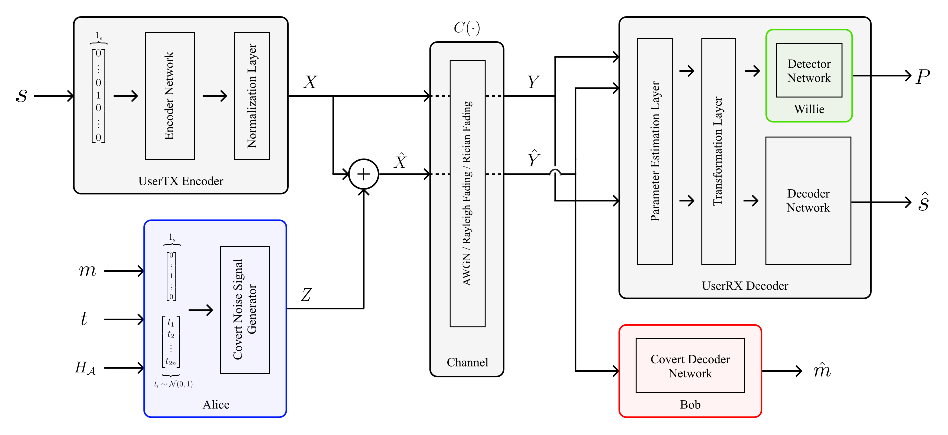
\includegraphics[width=\linewidth]{figs/system_architecture}
	\end{subfigure}
	\\
	\caption{Overall architecture of our system model. Alice communicating to Bob by generating covert noise signals without disturbing the normal communication between UserTX and UserRX; meanwhile Willie tries to distinguish covert and normal signals (Components under the control of covert users are colored and gray components are the persistent existing parts of the system).}	
	\label{fig:system_architecture}
\end{figure*}


\section{System Model}
\label{s:model}
In this section, we give an overall view of the system and define each actor's rule in our model. We also provide a brief background on autoencoder systems.


An overview of our system architecture is shown in figure (\ref{fig:system_architecture}). The system consists of two normal communication parties: normal sender (UserTX), normal receiver (UserRX) who are using an autoencoder model to communicate. The main objective of our work is to establish a covert channel on top of this normal communication without disturbing it. In this model, UserTX uses an encoder network to encode binary messages to a vector of signals. This vector of signals is then transmitted over the channel. We consider three channel models of AWGN, Rayleigh fading, and Rician fading. Signals passing through the channel get distorted by the channel's effect and a noisy version of them are received at the UserRX receiver. Eventually, using a decoder network, UserRX tries to extract the message from the received signals. The remaining three entities of our system are our covert actors. The objective of covert sender (Alice) is to secretly communicate with covert receiver (Bob) by embedding messages in form of perturbations that have similar statistical properties as of the channel's noise. Similar to any covert communication scheme, there is an observer (Willie) whose objective is to monitor the communication and recognize if any covert communication is taking place. All these three covert actors are collaborating and are represented by DNNs. Alice uses a generative model that embeds a confidential message into a covert noise vector. The produced covert signal has to have the lowest impact possible on the normal communication of the system and have enough power to be successfully decoded at Bob's receiver at the same time. This signal is then transmitted over the channel after being added to a normal signal. No matter the channel model, the procedure by which Alice and Bob establish a covert channel stays the same. Observer or warden of the system is responsible for detecting and mitigating any probable covert channel or abnormal communication between entities. Any deviation in the statistical properties of the channel would raise an alarm for the observer. Therefore, Alice and Bob incorporate a statistical undetectability constraint on the produced covert signals. This is achieved by covert users competing an observer (Willie), who is set to rigorously classify signals as covert and normal. As long as Alice succeeds in deceiving Willie to classify covert signals as normal, it is ensured that the added covert noise signals are distributed as the channel's real noise, thus are undetectable.


\textbf{Background on Autoencoder Systems}: An autoencoder-based wireless communication system is an end-to-end learning paradigm that abstracts out the coding and modulation components of a  traditional modular communication system by replacing the transmitter and receiver with DNNs. The encoder (transmitter) first uses a mapping to transform \(k\) bits of data into a message \(s\) where \(s \in \{1,...,M\}\) and \(M = 2^k\). Then it takes this transformed message as an input and generates a signal \(x = E(s) \in \mathbb{R}^{2n}\), which is a real valued vector. This \(2 \times n\) dimensional real valued vector can be treated as an \(n\) dimensional complex vector where \(n\) is the number of channel uses that are needed for the signal to be transmitted over. Then, the channel's noise effect \(z\), which is usually considered to be AWGN, is added to the signal vector. Thus, the received signal at the receiver, carrying the noise of the channel, can be expressed as \(y = x + z\). Rayleigh and Rician fading channels is used in case of existence of objects in the environment subjecting signals to fading. In this channel model, received signal is given by \(y = h \cdot x + z\), where \(h \sim \mathcal{CN}(0, 1)\) is the fading channel gain. Regardless of channel model, the decoder (receiver) applies the transformation \(D: \mathbb{R}^{2n} \rightarrow M \) to outputs the reconstructed version of the message \(s\), which is denoted as \(\hat{s} = D(y)\).

\section{Covert Channel Model}
For a given binary secret message \(m\), Alice first one-hot encodes the message and then uses its generator model to produce a covert noise signal \(\hat{z}\). This covert signal is then added to a vector of normal signal \(x\), which is carrying a message between UserTX and UserRX. Therefore, the covert signals before being transmitted over the channel can be denoted as:
\begin{equation}
	\hat{x} = x + \hat{z}.
\end{equation}
The signal is then transmitted over the channel. We mentioned that we assume the channel between sender and receiver to be AWGN or Rayleigh. Therefore, there will be two different channel outputs for these two different channel models. We express the distortions caused by the channel as a mapping function \(C(\cdot)\).\\


\textit{AWGN Channel Output}: For the AWGN channel model, the signal received at the receiver carries within itself the channel noise effect \(z \sim \mathcal{N}(0, \sigma_{chl}^2)\). Thus, the channel function \(C(\cdot)\) and final covert signal \(\hat{y}\) can be represented as:
\begin{equation}
	\hat{y} = C(\hat{x}) = \hat{x} + z.
\end{equation}


\textit{Rayleigh and Rician Fading Channel Output}: For the Rayleigh and Rician fading channel models, we consider a flat block fading channel where each codeword is assumed to be faded independently. Let \(h\) be the fading coefficient for transmitting the codeword \(\hat{x}\), then the channel function \(C(.)\) and and the final covert signal \(\hat{y}\) is given by:
\begin{equation}
	\hat{y} = C(\hat{x}) = h \cdot \hat{x} + z.
\end{equation}


On the receiver side, Bob receives a transmitted signal \(\hat{y}\) after the channel noise being added into it. He uses its decoder network to reconstruct the covert message \(\hat{m}\). Meanwhile, the UserRX uses the same signal to extract the normal message \(\hat{s}\), which is the reconstructed message of \(s\).


The statistical properties of signals transmitted over the channel are captured by Willie. His objective is to classify sequences of normal \(y\) and covert signals \(\hat{y}\) and provide useful feedback to Alice. This feedback helps Alice to modify the produced covert signals such that they are indistinguishable from normal transmitted signals. In other words, it ensures that both normal and covert signals have similar statistical properties.


\subsection{General Formulation}

The very first objective of our covert model is to have a working covert channel. To this end, Bob has to have a plausible accuracy in decoding covert messages that Alice sends through the covert signals \(\hat{y}\). As mentioned in previous section, Alice employs a generative model instead of an encoder model suggested by \cite{mohammed2021adversarial}. Using an encoder model to produce covert signal perturbations will map each covert message \(m\) to a single covert noise vector \(\hat{z}\). Inevitably, these deterministic covert perturbations can be detected and averaged out with ease by a careful observer or a defender as already shown in a work of Bahramali et al. \cite{bahramali2021robust} studying a relatable covert attack problem against autoencoder wireless networks.
\begin{algorithm}[tp!]
	\caption{Optimizing covert models algorithm}\label{alg:cap}
	\small
	\begin{algorithmic}
		\State $X \gets$ normal signals data
		\State $S, M \gets$ normal and covert messages sets
		\State $A, B, W \gets$ Alice, Bob, and Willie network functions
		\State $D \gets$ UserRX decoder network function
		\State $\mathcal{H} \gets$ cross entropy function
		\State $C \gets$ channel's remapping function
		\For{epoch $ep \in \{1 \ldots n_{epochs}$\}}
			\State $t \sim \mathcal{N}(0, 1)$
			\State $\mathcal{L}_{Willie} = H(C(X), C(A(M, t) + X))$
			\State Update $W$ to minimize $\mathcal{L}_{Willie}$
			\State $\mathcal{L}_{Bob} = H(C(A(M, t) + X), M)$
			\State Update $B$ to minimize $\mathcal{L}_{Bob}$
			\State $\mathcal{L}_{UserRX} \gets H(D(C(A(M, t) + X)), S)$
			\State
			$\mathcal{L}_{Alice} = \lambda_{Bob} \mathcal{L}_{Bob} + \lambda_{UserRX} \mathcal{L}_{UserRX} - \lambda_{Willie} \mathcal{L}_{Willie}$
			\State Update $A$ to minimize $\mathcal{L}_{Alice}$
		\EndFor
	\end{algorithmic}
\end{algorithm}
Thus, we use an stochastic generative model for Alice so that each covert message gets mapped to a set of different covert noise signals. Let \(A(\cdot)\) be the underlying function of Alice's generative model that takes a random trigger \(t \sim \mathcal{N}(0, 1)\) and a covert message \(m\) and produces a covert signal \(\hat{z}\) (the corresponding covert signal then can be denoted as \(\hat{z}_{m, t} = A(m, t)\)). Let also  \(B(\cdot)\) be the underlying function of the decoder network that Bob makes use of to reconstruct the covert message \(\hat{m}\). Then the reliability of communication between Alice and Bob is achieved using the below loss function:
\begin{equation}
	\begin{aligned} \label{bob_loss}
	\mathcal{L}_{Bob} & = \mathbb{E}_{m}[H(\hat{m}, m)] \\
	& = \mathbb{E}_{m}[H(B(\hat{y}), m)] \\ 
	& = \mathbb{E}_{m}[H(B(C(\hat{x}), m)] \\ 
	& = \mathbb{E}_{m}[H(B(C(A(m, t) + x)), m)].
	\end{aligned}
\end{equation}


where \(H(\cdot)\) is the cross entropy between the probability of reconstructed covert message \(\hat{m}\) and the actual covert message \(m\). This equation can be used for optimizing both Alice's and Bob's networks by freezing one or the other network's parameters iteratively. While (\ref{bob_loss}) ensures the communication accuracy, we also need to consider that the generated perturbations should leave no detrimental impact on the normal communication between UserTX and UserRX, otherwise causing an unexpected increase in the error rate of communication is deemed as an abnormal behavior by Willie. We apply this constraint by minimizing the autoencoder's loss function during Alice's training:
\begin{equation}
	\begin{aligned} \label{alice_user_loss}
	\mathcal{L}_{UserRX} & = \mathbb{E}_{m}[H(\hat{s}, s)] \\
	& = \mathbb{E}_{m}[H(D(\hat{y}), s)] \\
	& = \mathbb{E}_{m}[H(D(C(\hat{z} + x)), s)] \\
	& = \mathbb{E}_{m}[H(D(C(A(m, t) + E(s))), s)].
	\end{aligned}
\end{equation}
where \(D(\cdot)\) is UserRX's decoder network function, and \(E(\cdot)\) is the underlying function of the UserTX's encoder network. Note that both UserTX's encoder and UserRX's decoder networks are frozen during this training and only Alice's parameters are updated.


In our model, the observer entity or Willie, acts as the discriminator in GAN models \cite{goodfellow2014generative}. The so-called real and fake samples in GANs' discriminator network training process is here mapped to normal and covert signals, respectively. Thus, we express the loss function of Willie as:
\begin{equation}
	\begin{aligned} \label{willie_loss}
	\mathcal{L}_{Willie} & = \mathbb{E}_{m}[H(\hat{y}, y)] \\
	& = \mathbb{E}_{m}[H(C(\hat{x}), C(x))] \\
	& = \mathbb{E}_{m}[H(C(A(m,t) + x), C(x))].
	\end{aligned}
\end{equation}
where \(H(\cdot)\) here is the binary cross entropy between the covert signal \(\hat{y}\) and the normal signal \(y\). This white-box adversarial training against Alice's network ensures that Willie will be adequately trained to tell covert and non-covert signals apart. On the other hand, we do not want the covert signals that Alice produces to deviate from the statistical properties of the normal signals on the channel, otherwise it is likely that the observer of the channel detects and mitigates the covert communication. To achieve this undetectability property, we pose a new constraint on Alice's optimization function for maximizing Willie's uncertainty about his predictions. Having a regularizer as such helps Alice and Bob to form their covert communication in a way that is indistinguishable from the actual channel's noise, yet understandable by both. Altogether, Alice's loss function can be expressed as a weighted sum of three different objectives:
\begin{equation}
	\begin{array}{l} \label{alice_loss}
	\mathcal{L}_{Alice} = \lambda_{Bob} \mathcal{L}_{Bob} + \lambda_{UserRX} \mathcal{L}_{UserRX} - \lambda_{Willie} \mathcal{L}_{Willie}.
\end{array}
\end{equation}
where \(\lambda_{Bob}\), \(\lambda_{UserRX}\), and \(\lambda_{Willie}\) determine the importance of each objective for training Alice's network. Algorithm \ref{alg:cap} summarizes the procedure by which we train our covert models.

\subsection{Neural Network Architecture}
Before discussing the architecture of our neural network models, we need to state the focus of this work is not to introduce an autoencoder wireless network, so we only give a brief description on how this model works. A more detailed explanation of such a network can be found in the original paper \cite{o2017introduction}.


\textbf{Autoencoder's Network}: As proposed in the original autoencoder wireless communication paper, autoencoder model accepts a binary message \(s\) of size \(k\) bits and outputs a reconstructed version of it \(\hat{s}\). Figure \ref{fig:autoencoder_architecture} depicts the overall architecture of our autoencoder model. The encoder part of the model first one-hot encodes the message and then maps it to a vector of signals of size \(2 \times n\), where \(n\) is the number of channel uses. This transmitted signal is then given to a mapping function that applies the channel effects. On the receiver side, two layers of parameter estimation and transformation only becomes active if channel model is Rayleigh or Rician fading. In our model, transformation function is a simple division function that divides the received signal by the estimated channel fading coefficients by the parameter estimation. Note that more complex transformation functions can be used and are described in \cite{o2017introduction}, however optimizing the performance of autoencoder model is out of the scope of this article. Eventually, the transformed signal is fed to the decoder's network and the original normal message is reconstructed. 

\begin{figure}[tp!]
	\center
	\begin{subfigure}{0.5\textwidth}
		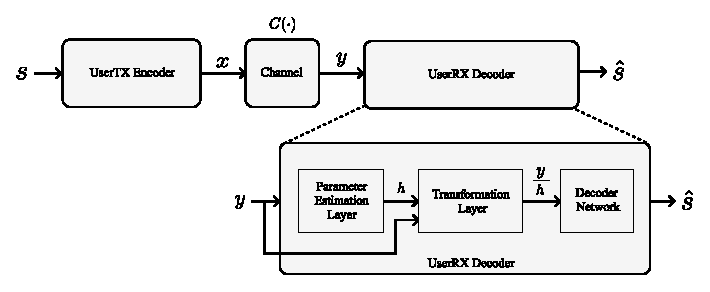
\includegraphics[width=\linewidth]{figs/autoencoder_architecture}
	\end{subfigure}
	\\
	\caption{Detailed architecture of UserRX's decoder network. Data passes through parameter estimation and transformation layers only when channel is Rayleigh or Rician.}	
	\label{fig:autoencoder_architecture}
\end{figure}

\begin{figure*}[!tp]
	\center
	\begin{subfigure}{0.3\textwidth}
		\includegraphics[width=\linewidth]{figs/autoencoder_bler_awgn}
		\caption{AWGN channel}
	\end{subfigure}
	\begin{subfigure}{0.3\textwidth}
		\includegraphics[width=\linewidth]{figs/autoencoder_bler_rayleigh}
		\caption{Rayleigh fading channel}	
	\end{subfigure}
	\begin{subfigure}{0.3\textwidth}
		\includegraphics[width=\linewidth]{figs/autoencoder_bler_rician}
		\caption{Rician fading channel}	
	\end{subfigure}
	\caption{Trained Autoencoder's BLER over a range of SNR values.}
	\label{fig:autoencoder_bler}
\end{figure*}

\textbf{Alice's Network}: Similar to the Autoencoder's encoder network, Alice takes a covert message \(m\) and transforms it to its corresponding one-hot encoding representation of it so that each message belongs to a unique class. Next, given a random trigger \(t\), Alice uses its generator model to produce a covert noise signal \(\hat{z}\) and then adds it to a normal signal \(x\) that is being transmitted at the time. For the Alice's generator model, we use multiple dense layers with ReLU and Tanh activation functions. The first layer of this model takes a trigger number \(t\) and an one-hot encoded covert message \(m\), and acts as embedding layer by enlarging the input's domain space. The following fully contacted layers are to extract the useful features and do the encoding process. The last layer of this model does a dimension transformation so that the generated covert signal \(\hat{z}\) complies with the dimension of the normal signal \(x\) on the channel. 

\textbf{Bob's Network}: Bob receives this covert signal \(\hat{y}\) that has undergone the channel's effects and feeds it through its decoder network regardless of what the channel model is and extracts the secret message by doing classification on the signal. Bob's network has a more complicated structure comparing to Alice as it has to decode the secret message from a signal \(\hat{y}\) that has been distorted stiffly as a result of going through the channel. The received message by Bob first goes through the first layer of the network, which is a wide dense layer with a Tanh activation function, to increase the input's feature space. Then the data is passed through multiple 1-Dimensional Convolutional (1D Conv) layers that supposedly learn the coding that Alice has fabricated to encode the covert messages. We have found that using 1D Conv layers helps Bob and Alice achieving a better consistency in the accuracy of their communication, especially when the channel model is more complicated (i.e. when there is also fading in the channel). The rest of Bob's decoder network consists of two dense layers that does a domain remapping from the learned feature space to the covert message domain space. Similar to the UserRX's decoder network, Bob eventually predicts the covert message by doing a classification on the received signal.


\textbf{Willie's Network}: Willie receives both the covert signal \(\hat{y}\) and the normal signal \(y\) and outputs a confidence probability \(P\) on how probable it is for the signal to be normal. We choose the same network architecture of Bob's for Willie except for the last layer that has a Sigmoid activation function instead of Softmax. This ensures that Bob and Willie has the same capacity of training and can be compete each other in a fair setup.


\begin{table}[tp!]
	\begin{adjustbox}{width=0.85\columnwidth,center}
		\begin{tabular}{|l|l|} 
			\hline
			\multicolumn{2}{|c|}{\textbf{Alice}} 															\\
			\hline
			Layer 																	&	Output dimension	\\
			\hline
			Input (size 8 + $2^k$)      											&	-    	 		    \\ 
			Dense + ReLU          													&	32 + $2^{k+1}$		\\
			Dense + ReLU          													&	32 + $2^{k+1}$		\\
			Dense + ReLU   															&	8 $\times$ $2^k$	\\
			Dense																	&	8 $\times$ 2	\\
			\hline   
			\hline												
			\multicolumn{2}{|c|}{\textbf{Bob, Willie}} 											\\
			\hline
			Input (size 2 $\times$ 8)
			Dense + Tanh																&	2 $\times$ 8			\\
			Convolutional (8 filters, kernel size 1 $\times$ 1, stride 1) + LeakyReLU 	&   8 $\times$ 16			\\
			Convolutional (8 filters, kernel size 1 $\times$ 2, stride 1) + LeakyReLU 	&   8 $\times$ 15			\\
			Convolutional (8 filters, kernel size 1 $\times$ 4, stride 2) + LeakyReLU 	&   8 $\times$ 6			\\
			Convolutional (8 filters, kernel size 1 $\times$ 2, stride 1) + LeakyReLU 	&   8 $\times$ 5			\\
			Convolutional (8 filters, kernel size 1 $\times$ 2, stride 1) + LeakyReLU 	&   8 $\times$ 4			\\
			Flatten															 			&   32						\\
			Dense + Tanh																&	16						\\
			Dense + (Willie: Sigmoid, Bob: Softmax)										&	Willie: 1, Bob:	$2^k$	\\
			\hline
		\end{tabular}
	\end{adjustbox}
	\caption{Alice, Bob, and Willie's networks detailed architecture.}
	\label{table:covert_models_structure}
\end{table}

\begin{table}[tp!]
	\begin{adjustbox}{width=0.85\columnwidth,center}
		\begin{tabular}{|l|l|} 
			\hline
			\multicolumn{2}{|c|}{\textbf{Encoder}} 															\\
			\hline
			Layer 																	&	Output dimension	\\
			\hline
			Input (size 16)      												&	-    	 		    \\ 
			Dense + ELU          													&	16					\\
			Dense + ELU   															&	2 $\times$ 8		\\
			Convolutional (8 filters, kernel size 1 $\times$ 2, stride 1) + Tanh 	&   8 $\times$ 15		\\
			Convolutional (8 filters, kernel size 1 $\times$ 4, stride 2) + Tanh 	&   8 $\times$ 6		\\
			Convolutional (8 filters, kernel size 1 $\times$ 2, stride 1) + Tanh 	&   8 $\times$ 5		\\
			Convolutional (8 filters, kernel size 1 $\times$ 2, stride 1) + Tanh 	&   8 $\times$ 4		\\
			Flatten															 		&   32					\\
			Dense																	&	2 $\times$ 8		\\
			Normalization															&	2 $\times$ 8		\\
			\hline   
			\hline												
			\multicolumn{2}{|c|}{\textbf{Parameter Estimation}} 											\\
			\hline
			Dense + ELU																&	2 $\times$ 16		\\
			Dense + Tanh															&	2 $\times$ 32		\\
			Dense + Tanh															&	2 $\times$ 8		\\
			Dense																	&	2 $\times$	1		\\
			\hline
			\hline
			\multicolumn{2}{|c|}{\textbf{Decoder}}															\\
			\hline
			Layer 																	&	output dimension	\\
			\hline
			Dense + Tanh          													&	2 $\times$ 8		\\
			Convolutional (8 filters, kernel size 1 $\times$ 2, stride 1) + Tanh 	&   8 $\times$ 15		\\
			Convolutional (8 filters, kernel size 1 $\times$ 4, stride 2) + Tanh 	&   8 $\times$ 6		\\
			Convolutional (8 filters, kernel size 1 $\times$ 2, stride 1) + Tanh 	&   8 $\times$ 5		\\
			Convolutional (8 filters, kernel size 1 $\times$ 2, stride 1) + Tanh 	&   8 $\times$ 4		\\
			Flatten															 		&   32					\\
			Dense + Tanh															&	2 $\times$ 8		\\
			Dense + Tanh															&	2 $\times$ 8		\\
			Dense + Softmax															&	16					\\ 
			\hline
		\end{tabular}
	\end{adjustbox}
	\caption{Autoencoder's network detailed architecture.}
	\label{table:autoencoder_structure}
\end{table}